% !TeX root = ../../thesis.tex

\section{\acs{UEFI} Shell}

Part of the family of \ac{UEFI} specifications is a shell specification which defines a feature rich \ac{UEFI} shell application to interact with the \ac{UEFI} environment \cite[Section 1.1]{uefi-shell-spec}.
It offers commands relating to boot and general configuration, device and driver management, file system access, networking \cite[Section 5.1]{uefi-shell-spec} and scripting \cite[Section 4]{uefi-shell-spec}.
A shell application may already be part of the boot options but can always be supplied in the default boot path of removable media.

The \ac{UEFI} shell is a great tool to visualize the \ac{UEFI} environment.
With the \program{devtree} command, for example, we can see the tree of all handles complying to the \ac{UEFI} driver model.
This also serves a great reference of how device paths are formed.
\autoref{fig:devtree} shows the output of \program{devtree} cropped to show a \ac{GPT} formatted hard drive and its logical partitions.
When the firmware discovers a block device it is also required to search for a partition table and create a device handle for each partition.
Device drivers abstracting file systems can then be connected to a partition handle and check if it is formatted.
The first partition here, listed as \emph{FAT File System}, is the \ac{ESP} of this drive.

\begin{figure}[htb]
    \centering
    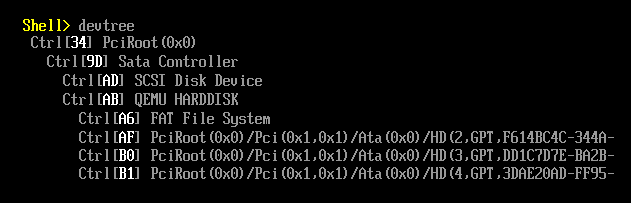
\includegraphics[width=1.0\textwidth]{uefi/devtree}
    \caption{Shortened \ac{UEFI} shell output of \program{devtree}}
    \label{fig:devtree}
\end{figure}

With \program{openinfo} we can see the group of protocols that a handle represents.
\autoref{fig:openinfo} shows the output when querying the handle of an \ac{ESP}.
Since this \ac{ESP} is installed in a logical partition an instance of the Partition Information Protocol is present.
The command also lists the agent handles of each protocol and how the protocol was accessed.
\code{TestProt} is often used in the \code{Supported} function of a driver, while \code{GetProt} is then used to open the protocol for consumption within the \code{Start} function.

\begin{figure}[htb]
    \centering
    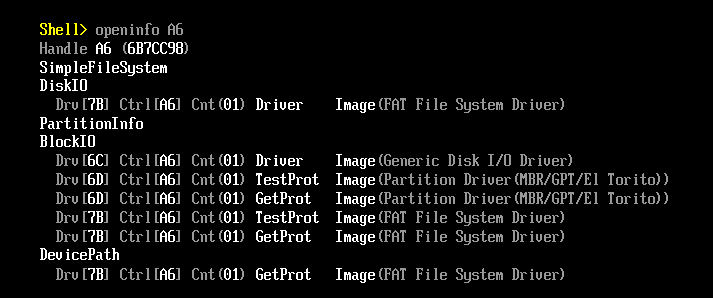
\includegraphics[width=1.0\textwidth]{uefi/openinfo}
    \caption{Shortened \ac{UEFI} shell output of \program{openinfo}}
    \label{fig:openinfo}
\end{figure}



% During initialization the shell produces default mappings for file systems and block devices, this defines names that can be used interchangably with their device paths when issuing shell commands \cite[Section 3.7.2]{uefi-shell-spec}.
% These mappings are designed to be consistent across reboots as long as the hardware configuration stays the same, they are comparable to Windows partition letters \cite[Appendix A]{uefi-shell-spec}.
% It also produces the initial output of what is equivalent to the invocation of the commands \program{ver} and \program{map} \cite[Section 3.3]{uefi-shell-spec}.
% \program{ver} displays the version of the \ac{UEFI} specification the firmware conforms to, while map shows the current device mapping \cite[Section 5.3]{uefi-shell-spec}.
% \autoref{fig:uefi-shell} depicts an exemplary output of the \ac{EDK} II \ac{UEFI} shell.

% When we inspect the mapping table we can see \lstinline{FSx:} and \lstinline{BLKx:} aliases, \lstinline{FSx:} maps to file systems and \lstinline{BLKx:} to block devices.
% This identification is performed via instances of the \hyperref[lst:simple-file-system-protocol]{Simple File System Protocol} and \TODO{double check} Block \ac{I/O} Protocol.
% % explain Simple File System Protocol
% The \hyperref[lst:simple-file-system-protocol]{Simple File System Protocol} \cite[Section 13.4]{uefi-spec} provides, together with the \hyperref[lst:simple-file-system-protocol]{File Protocol}, file-type access to the device it is installed on \cite[Section 13.5]{uefi-spec}.
% The two protocols are independent of the underlying file system the media is formatted with.
